\chapter{\ifproject%
\ifcpe โครงสร้างและขั้นตอนการทำงาน\else Project Structure and Methodology\fi
\else%
\ifcpe โครงสร้างของโครงงาน\else Project Structure\fi
\fi
}

% ในบทนี้จะกล่าวถึงหลักการ และการออกแบบระบบ

\makeatletter

% \renewcommand\section{\@startsection {section}{1}{\z@}%
%                                    {13.5ex \@plus -1ex \@minus -.2ex}%
%                                    {2.3ex \@plus.2ex}%
%                                    {\normalfont\large\bfseries}}

\makeatother
%\vspace{2ex}
% \titleformat{\section}{\normalfont\bfseries}{\thesection}{1em}{}
% \titlespacing*{\section}{0pt}{10ex}{0pt}

\section{User Interface (UI)}
User interface (UI) คือ การออกแบบที่เน้นไปที่เรื่องหน้าตา ความสวยงาม และทุกอย่างที่จะเป็นการโต้ตอบกับผู้ใช้งาน โดยจะแสดงการเชื่อมโยงของแต่ละหน้าผ่าน User Flow ดังรูปที่ \ref{userflow} UI ที่ดีจะช่วยดึงดูดผู้ใช้งานให้เกิดความสนใจและช่วยให้ผู้ใช้งานเข้าถึงข้อมูลได้ง่าย
โดยการออกแบบ UI ของเกมนี้พวกเราจะออกแบบเกมแนวตะลุยไปยังแผนที่ต่างๆที่มีสภาพแวดล้อมแตกต่างกัน โดยจะใช้ Asset ที่มีอยู่ใน Unity มาปรับแต่งจัดวางเพื่อความสวยงามและความน่าสนใจ โดยจะมีส่วนต่างๆ ดังนี้ ซึ่งจะแสดงดังรูปต่อไปนี้
\begin{itemize}
\item หน้าจอแสดง Mainmenu รูปที่ \ref{mainmenu}
\item หน้าจอแสดงหน้าเลือกแผนที่ รูปที่ \ref{map}
\item หน้าจอแสดงหน้าเลือกด่าน รูปที่ \ref{stage}
\item หน้าจอแสดงหน้า Gameplay รูปที่ \ref{game}
\item หน้าต่างที่แสดงว่าเราชนะ รูปที่ \ref{win}
\item หน้าต่างที่แสดงว่าเราแพ้ รูปที่ \ref{lose}
\end{itemize}

\section{WebView}
ตัวหน้าเว็ปทำขึ้นมาเพื่อนำ Google Blockly ไปใส่ใน panel ของ Unity เพราะเดิมที Unity ไม่สามารถสร้าง Object ที่หน้าตาและรวมไปถึง function ที่เหมือนกับ Google Blockly ได้ ทางผู้พัฒนาเลยสร้างหน้าเว็ปเข้ามาเพื่อนำไปใส่ใน 
panel ของ Unity ที่ใช้ในการแสดงผล Block Code

\section{Text Reader}
การสร้างด่านของเกมนี้จะ Input ด้วยไฟล์ Text กล่าวคือเมื่อ User ทำการ Input ไฟล์มาตัวระบบเกมจะทำการจัดการสร้างด่านให้เอง
ทำให้การที่จะสร้างด่านหนึ่งด่านไม่ต้องทานั่งลากวางตัว prefabs บน Unity ตัวอย่างไฟล์ Text คร่าวๆ จากรูป \ref{txt}

\begin{figure}[h!]
\begin{center}
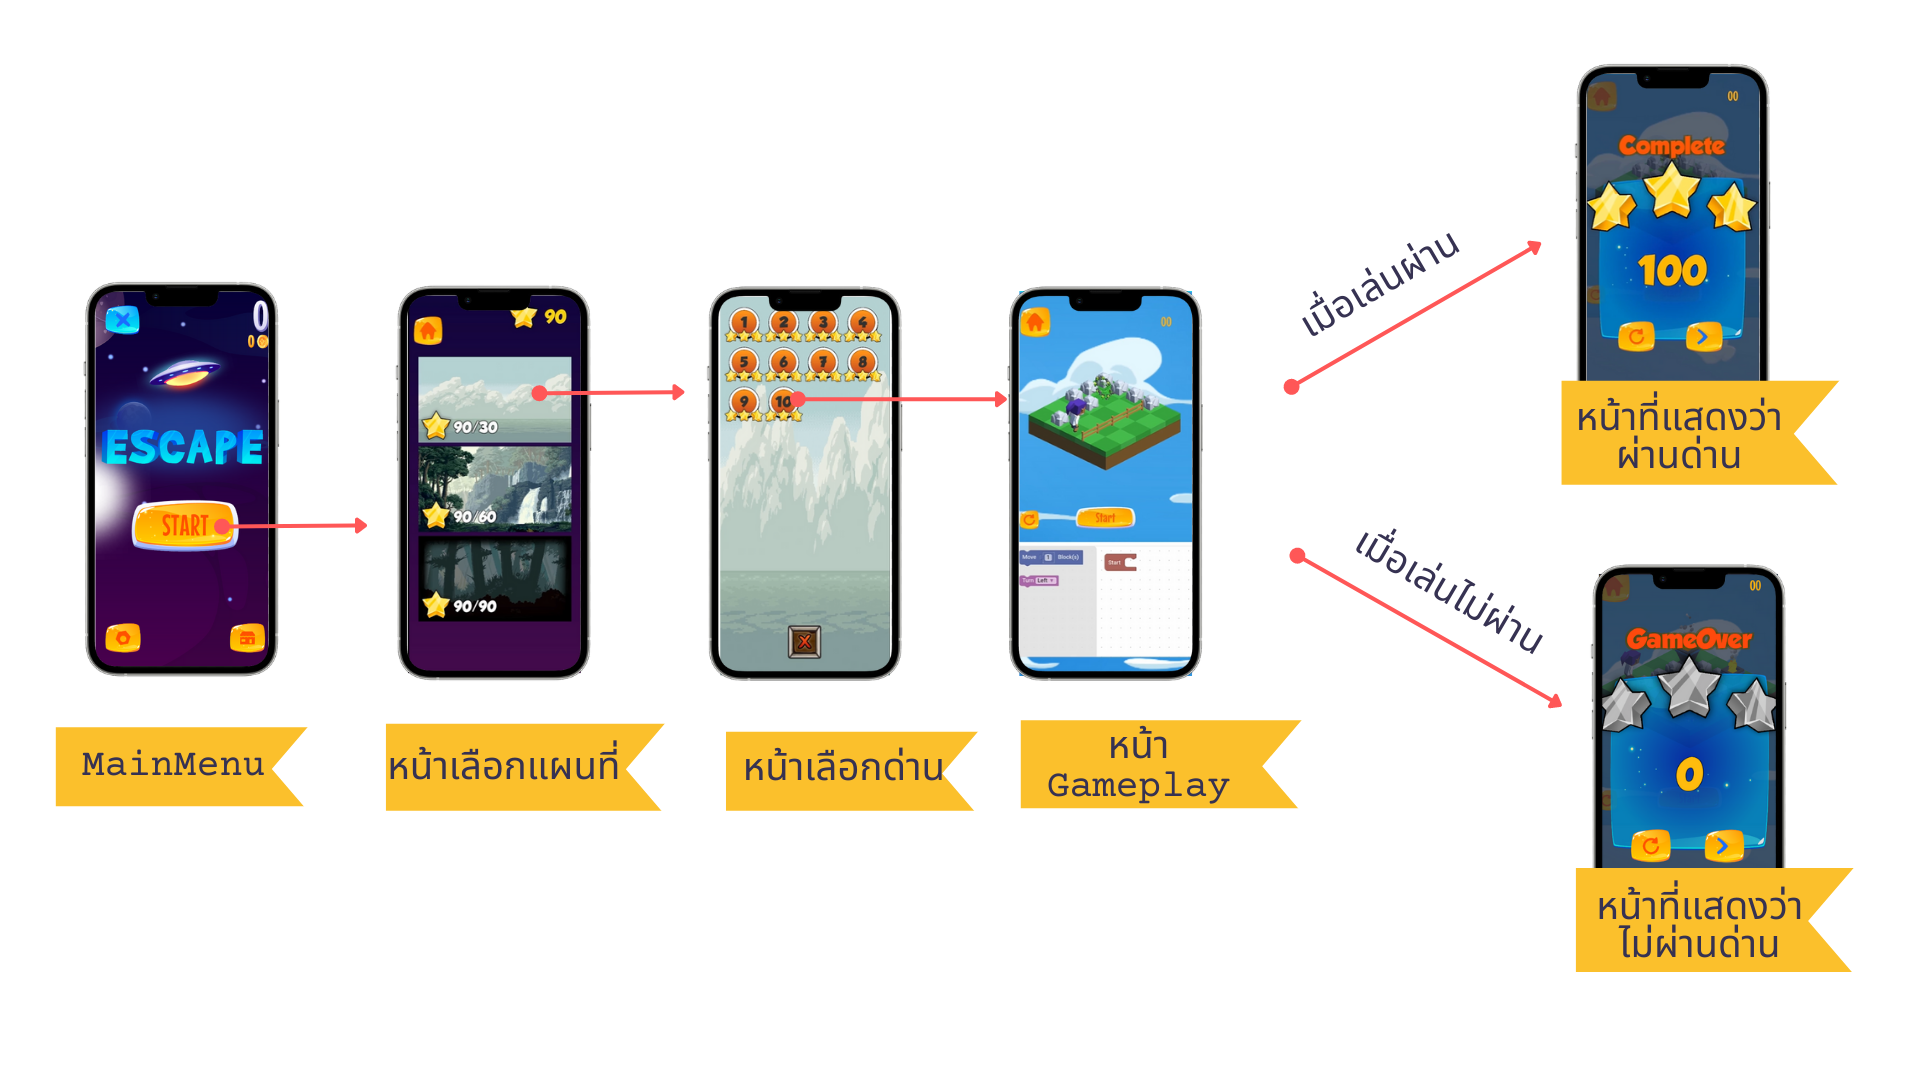
\includegraphics [scale=.35] {pic/UXflowchart.png}
\end{center}
\caption[User Flow]{User Flow}
\label{userflow}
\end{figure}


\GBreply{ควรจะเอาขึ้นก่อนไหม? อธิบายด้วย ไม่ใช่ว่าแปะๆๆ อาจจะทำ User Flow ไหม?}
\begin{figure}[h!]
\begin{center}
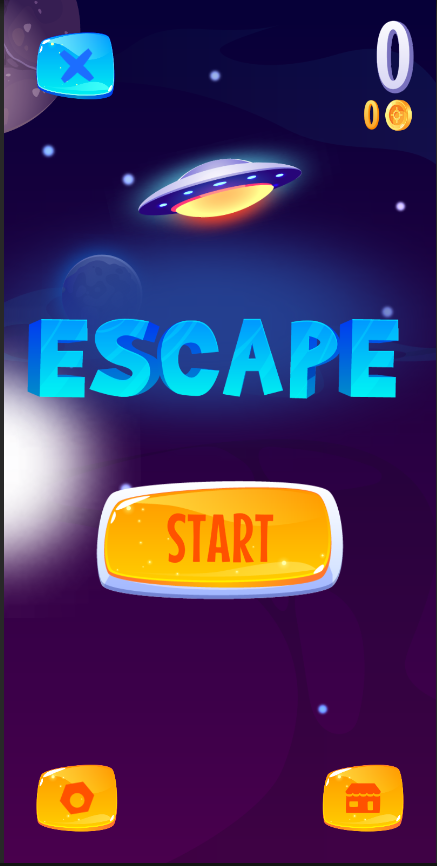
\includegraphics[scale = 0.4]{pic/home_start.PNG}
\end{center}
\caption[Mainmenu ของเกม]{หน้า Mainmenu ของเกม}
\label{mainmenu}
\end{figure}


\begin{figure}[h!]
\begin{center}
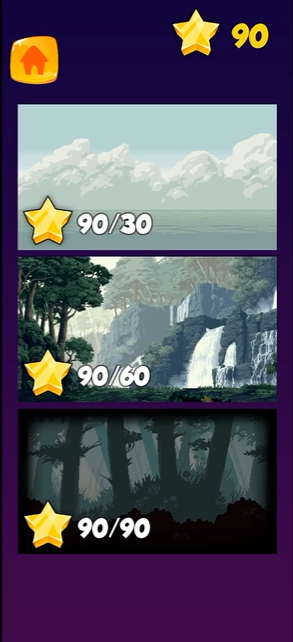
\includegraphics[scale = 0.5]{pic/MapSelection.png}
\end{center}
\caption[หน้าเลือกแผนที่]{หน้าเลือกแผนที่}
\label{map}
\end{figure}

\begin{figure}[h!]
\begin{center}
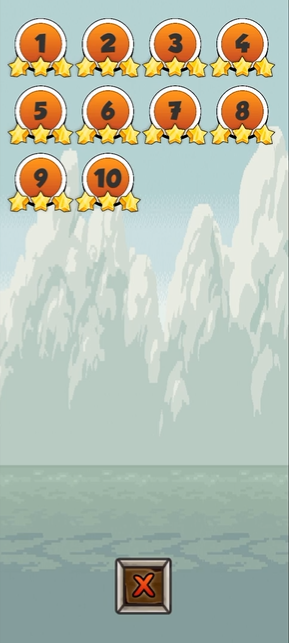
\includegraphics[scale = 0.5]{pic/LevelSelection1.png}
\end{center}
\caption[หน้าเลือกด่าน]{หน้าเลือกด่าน}
\label{stage}
\end{figure}


\begin{figure}[h!]
\begin{center}
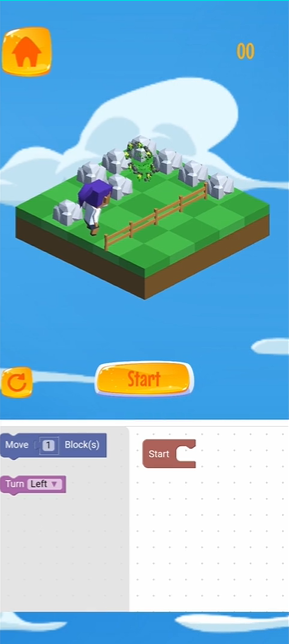
\includegraphics[scale = 0.5]{pic/NewGamePlay.png}
\end{center}
\caption[หน้า Gameplay]{หน้า Gameplay}
\label{game}
\end{figure}

\begin{figure}[h!]
\begin{center}
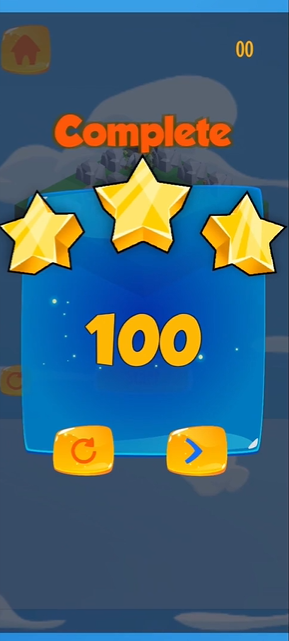
\includegraphics[scale = 0.5]{pic/Complete.png}
\end{center}
\caption[หน้าต่างที่แสดงว่าชนะ]{หน้าต่างที่แสดงว่าชนะ}
\label{win}
\end{figure}

\begin{figure}[h!]
\begin{center}
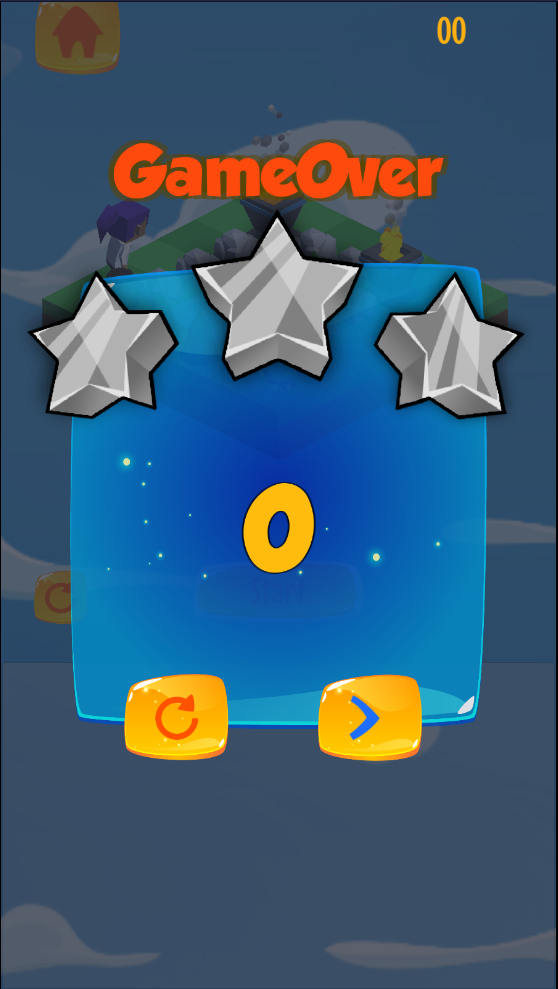
\includegraphics[scale = 0.3]{pic/GameOver1.png}
\end{center}
\caption[หน้าต่าง GameOver]{หน้าต่าง GameOver}
\label{lose}
\end{figure}


\begin{figure}[h!]
\begin{center}
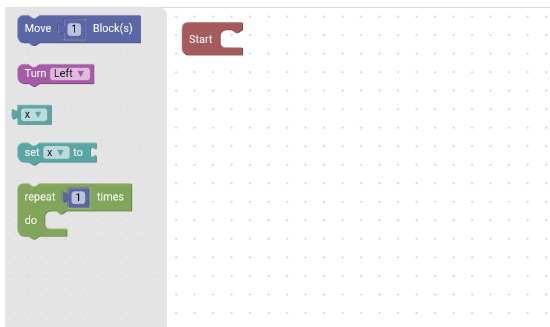
\includegraphics{pic/CodePanel.png}
\end{center}
\caption[Google Blockly]{Google Blockly}
\label{block}
\end{figure}


\begin{figure}[h!]
    \begin{center}
    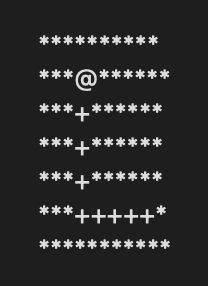
\includegraphics{pic/text.png}
    \end{center}
    \caption[Text]{Text}
    \label{txt}
    \end{figure}
